% CH4114 — Tutorial 00, Part 3: uv Environments
% Beamer deck, 16:9, compiled with pdflatex (TeX Live 2026)
% Author: Shuvam Banerji Seal
\documentclass[aspectratio=169]{beamer}

\usetheme{Madrid}
\usecolortheme{whale}
\setbeamertemplate{navigation symbols}{}

\usepackage[T1]{fontenc}
\usepackage{tikz}
\usetikzlibrary{arrows.meta, positioning}
\usepackage{booktabs}
\usepackage{listings}
\lstset{
  basicstyle=\ttfamily\footnotesize,
  breaklines=true,
  showstringspaces=false,
  columns=fullflexible,
  keepspaces=true,
}

\title[uv Environments]{Tutorial 00 --- Part 3\\[2pt] uv: Python Environments Without the Pain}
\subtitle{init, add, sync, run --- the whole lifecycle}
\author[SBS]{Shuvam Banerji Seal}
\institute[CH4114]{CH4114 --- Molecular Simulation}
\date[Aug 2026]{14 August 2026}

\begin{document}

% ------------------------------------------------------------------ title
\begin{frame}[plain]
  \titlepage
  \centering{\scriptsize Course Instructor: Dr.\ Susmita Roy \quad$\cdot$\quad TA: Shuvam Banerji Seal}\par
  \vspace{0.1cm}
  \centering{\scriptsize Repository: \texttt{CH4114\_Molecular\_Simulation\_Tutorials}}
\end{frame}

% ---------------------------------------------------------------- problem
\begin{frame}[fragile]{The problem uv solves}
  \begin{columns}[T]
    \begin{column}{0.5\textwidth}
      \begin{block}{The old way}
        \begin{lstlisting}
python -m venv .venv
source .venv/bin/activate
pip install numpy mdtraj
pip freeze > requirements.txt
        \end{lstlisting}
      \end{block}
    \end{column}
    \begin{column}{0.46\textwidth}
      \begin{itemize}
        \item \texttt{pip freeze} captures your \emph{whole machine}, not the project.
        \item No Python version, no platform, no dev-vs-runtime split.
        \item Environments rot; ``works on my machine''.
      \end{itemize}
    \end{column}
  \end{columns}
  \vspace{0.2cm}
  \begin{block}{uv (by Astral)}
    One fast binary that manages interpreters, environments, dependencies,
    locking, and tools. 10--100$\times$ faster than pip.
  \end{block}
\end{frame}

% ------------------------------------------------------------ what replaces
\begin{frame}{What uv replaces}
  \begin{table}
    \small
    \begin{tabular}{@{}lll@{}}
      \toprule
      Old tool & Job & uv command \\
      \midrule
      \texttt{python -m venv} & create env & \texttt{uv venv} / \texttt{uv sync} \\
      \texttt{pip install} & add packages & \texttt{uv add} \\
      \texttt{pip uninstall} & remove packages & \texttt{uv remove} \\
      \texttt{requirements.txt} & pin versions & \texttt{uv.lock} \\
      \texttt{pyenv} & manage Pythons & \texttt{uv python install} \\
      \texttt{pip freeze} & snapshot env & \texttt{uv lock} \\
      \texttt{npx}-style tools & run tools & \texttt{uvx} \\
      \bottomrule
    \end{tabular}
  \end{table}
  \vspace{0.3cm}
  \begin{itemize}
    \item One mental model, one tool, one lockfile.
  \end{itemize}
\end{frame}

% ------------------------------------------------------------ installation
\begin{frame}[fragile]{Installation on every OS}
  \begin{columns}[T]
    \begin{column}{0.32\textwidth}
      \begin{block}{Linux}
        \begin{lstlisting}
curl -LsSf https://astral.sh/
  uv/install.sh | sh
# or: sudo apt install uv
        \end{lstlisting}
      \end{block}
    \end{column}
    \begin{column}{0.32\textwidth}
      \begin{block}{macOS}
        \begin{lstlisting}
curl -LsSf https://astral.sh/
  uv/install.sh | sh
# or: brew install uv
        \end{lstlisting}
      \end{block}
    \end{column}
    \begin{column}{0.32\textwidth}
      \begin{block}{Windows}
        \begin{lstlisting}
powershell -ExecutionPolicy
  ByPass -c "irm https://
  astral.sh/uv/install.sh | iex"
# or: winget install
#     --id=astral-sh.uv
        \end{lstlisting}
      \end{block}
    \end{column}
  \end{columns}
  \vspace{0.2cm}
  \begin{center}
    Verify everywhere: \texttt{uv --version}
  \end{center}
\end{frame}

% ------------------------------------------------------------------ path
\begin{frame}[fragile]{If \texttt{uv: command not found}: fix your PATH}
  \begin{columns}[T]
    \begin{column}{0.48\textwidth}
      \begin{block}{Bash --- \texttt{\textasciitilde/.bashrc}}
        \begin{lstlisting}
export PATH="$HOME/.local/bin:$PATH"
        \end{lstlisting}
        \begin{lstlisting}
source ~/.bashrc
        \end{lstlisting}
      \end{block}
    \end{column}
    \begin{column}{0.48\textwidth}
      \begin{block}{Zsh --- \texttt{\textasciitilde/.zshrc}}
        \begin{lstlisting}
export PATH="$HOME/.local/bin:$PATH"
        \end{lstlisting}
        \begin{lstlisting}
source ~/.zshrc
        \end{lstlisting}
      \end{block}
    \end{column}
  \end{columns}
  \vspace{0.2cm}
  \begin{itemize}
    \item Installer puts uv in \texttt{\textasciitilde/.local/bin} (Homebrew: \texttt{/opt/homebrew/bin}).
    \item Verify: \texttt{which uv} and \texttt{uv --version} in a fresh terminal.
  \end{itemize}
\end{frame}

% ------------------------------------------------------------ main commands
\begin{frame}{The main commands of this session}
  \begin{center}
    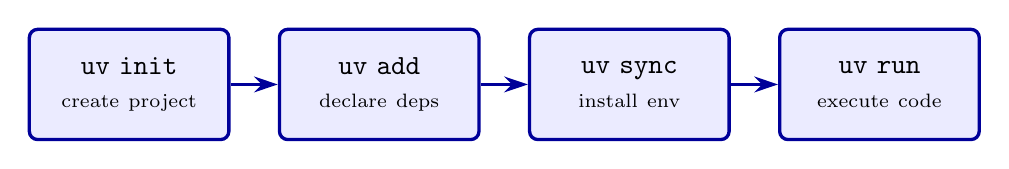
\begin{tikzpicture}[
        s/.style={rectangle, draw=blue!60!black, very thick, rounded corners=3pt,
                  fill=blue!8, text width=2.3cm, align=center,
                  minimum height=1.4cm},
        arr/.style={-{Stealth[length=3mm,width=2mm]}, very thick, blue!60!black},
        node distance=0.6cm]
      \node[s] (init) {\texttt{uv init}\\ {\scriptsize create project}};
      \node[s, right=of init] (add) {\texttt{uv add}\\ {\scriptsize declare deps}};
      \node[s, right=of add] (sync) {\texttt{uv sync}\\ {\scriptsize install env}};
      \node[s, right=of sync] (run) {\texttt{uv run}\\ {\scriptsize execute code}};
      \draw[arr] (init) -- (add);
      \draw[arr] (add) -- (sync);
      \draw[arr] (sync) -- (run);
    \end{tikzpicture}
  \end{center}
  \vspace{0.2cm}
  \begin{center}
    \small
    \texttt{uv init demo \&\& cd demo}\quad
    \texttt{uv add numpy mdtraj}\quad
    \texttt{uv sync}\quad
    \texttt{uv run python -c "import numpy"}
  \end{center}
  \begin{itemize}
    \item That is the entire lifecycle of a Python project in four commands.
  \end{itemize}
\end{frame}

% ------------------------------------------------------------ two files
\begin{frame}{The two-file contract}
  \begin{center}
    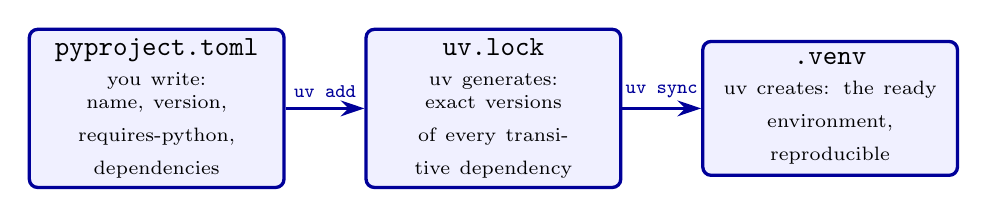
\begin{tikzpicture}[
        b/.style={rectangle, draw=blue!60!black, very thick, rounded corners=3pt,
                  fill=blue!6, text width=3.0cm, align=center,
                  minimum height=1.7cm},
        arr/.style={-{Stealth[length=3mm,width=2mm]}, very thick, blue!60!black},
        lab/.style={font=\scriptsize\ttfamily},
        node distance=1.0cm]
      \node[b] (pp) {\texttt{pyproject.toml}\\[3pt] {\scriptsize you write: name, version,\\ requires-python, dependencies}};
      \node[b, right=of pp] (lk) {\texttt{uv.lock}\\[3pt] {\scriptsize uv generates: exact versions\\ of every transitive dependency}};
      \node[b, right=of lk] (venv) {\texttt{.venv}\\[3pt] {\scriptsize uv creates: the ready\\ environment, reproducible}};
      \draw[arr] (pp) -- node[lab, above] {uv add} (lk);
      \draw[arr] (lk) -- node[lab, above] {uv sync} (venv);
    \end{tikzpicture}
  \end{center}
  \vspace{0.3cm}
  \begin{itemize}
    \item Commit \textbf{both} files: \texttt{uv.lock} is the reproducibility contract.
    \item Anyone running \texttt{uv sync} gets byte-identical dependencies.
  \end{itemize}
\end{frame}

% ---------------------------------------------------------------- uv init
\begin{frame}[fragile]{uv init: what you get}
  \begin{columns}[T]
    \begin{column}{0.45\textwidth}
      \begin{lstlisting}
uv init my_project
cd my_project
      \end{lstlisting}
    \end{column}
    \begin{column}{0.5\textwidth}
      \begin{lstlisting}
my_project/
+-- .python-version
+-- README.md
+-- pyproject.toml
+-- src/my_project/
|   +-- __init__.py
|   +-- main.py
+-- .gitignore
      \end{lstlisting}
    \end{column}
  \end{columns}
  \vspace{0.2cm}
  \begin{itemize}
    \item A ready-to-run project: metadata, package, gitignore, pinned Python.
    \item \texttt{uv run python src/my\_project/main.py} prints the hello world.
  \end{itemize}
\end{frame}

% ---------------------------------------------------------------- uv sync
\begin{frame}[fragile]{uv sync and uv run}
  \begin{columns}[T]
    \begin{column}{0.48\textwidth}
      \begin{block}{uv sync}
        \begin{lstlisting}
uv sync
        \end{lstlisting}
        \begin{itemize}
          \item creates \texttt{.venv/}
          \item resolves dependencies
          \item writes \texttt{uv.lock}
          \item installs the project (editable)
        \end{itemize}
      \end{block}
    \end{column}
    \begin{column}{0.48\textwidth}
      \begin{block}{uv run --- no activation needed}
        \begin{lstlisting}
uv run python script.py
uv run pytest
uv run python -c "import numpy"
        \end{lstlisting}
      \end{block}
      \begin{itemize}
        \item \texttt{uv run} uses the project environment automatically.
        \item Manual activation still works:
              \texttt{source .venv/bin/activate}.
      \end{itemize}
    \end{column}
  \end{columns}
\end{frame}

% ---------------------------------------------------------------- uv add
\begin{frame}[fragile]{uv add and uv remove}
  \begin{columns}[T]
    \begin{column}{0.5\textwidth}
      \begin{block}{Commands}
        \begin{lstlisting}
uv add numpy
uv add "numpy>=2.0"
uv add mdtraj matplotlib
uv add --dev pytest
uv remove mdtraj
        \end{lstlisting}
      \end{block}
    \end{column}
    \begin{column}{0.46\textwidth}
      \begin{block}{pyproject.toml after uv add}
        \begin{lstlisting}
[project]
dependencies = [
    "mdtraj>=1.10",
    "numpy>=2.0",
]

[dependency-groups]
dev = [
    "pytest>=8.0",
]
        \end{lstlisting}
      \end{block}
    \end{column}
  \end{columns}
  \vspace{0.2cm}
  \begin{itemize}
    \item \texttt{uv add} edits \texttt{pyproject.toml} \emph{and} \texttt{uv.lock},
          then syncs --- three pip steps in one.
  \end{itemize}
\end{frame}

% ---------------------------------------------------------------- uvx
\begin{frame}[fragile]{Running tools: uv run and uvx}
  \begin{columns}[T]
    \begin{column}{0.48\textwidth}
      \begin{block}{uv run --- project tools}
        \begin{lstlisting}
uv run python script.py
uv run pytest
uv run ruff check .
        \end{lstlisting}
      \end{block}
    \end{column}
    \begin{column}{0.48\textwidth}
      \begin{block}{uvx --- ephemeral tools}
        \begin{lstlisting}
uvx ruff check .
uvx black --check .
uvx mamba --help
        \end{lstlisting}
      \end{block}
    \end{column}
  \end{columns}
  \vspace{0.2cm}
  \begin{itemize}
    \item \texttt{uvx} runs a tool in a throwaway environment --- nothing
          pollutes your project.
  \end{itemize}
\end{frame}

% ------------------------------------------------------------ reproducing
\begin{frame}{Reproducing someone else's project}
  \begin{center}
    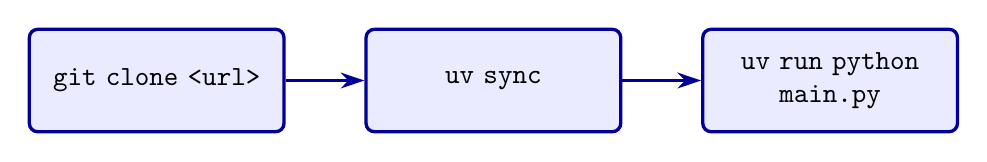
\begin{tikzpicture}[
        b/.style={rectangle, draw=blue!60!black, very thick, rounded corners=3pt,
                  fill=blue!8, text width=3.0cm, align=center,
                  minimum height=1.3cm},
        arr/.style={-{Stealth[length=3mm,width=2mm]}, very thick, blue!60!black},
        node distance=1.0cm]
      \node[b] (clone) {\texttt{git clone <url>}};
      \node[b, right=of clone] (sync) {\texttt{uv sync}};
      \node[b, right=of sync] (run) {\texttt{uv run python main.py}};
      \draw[arr] (clone) -- (sync);
      \draw[arr] (sync) -- (run);
    \end{tikzpicture}
  \end{center}
  \vspace{0.3cm}
  \begin{block}{The result}
    Same lockfile $\rightarrow$ same environment $\rightarrow$
    ``works on my machine'' is dead. \quad
    Upgrades: \texttt{uv lock --upgrade} then \texttt{uv sync}.
  \end{block}
\end{frame}

% ------------------------------------------------------------ reference
\begin{frame}{uv command reference}
  \begin{table}
    \scriptsize
    \begin{tabular}{@{}ll@{}}
      \toprule
      Command & What it does \\
      \midrule
      \texttt{uv init [name]} & scaffold a new project \\
      \texttt{uv sync} & create env + install deps from lockfile \\
      \texttt{uv add <pkg>} / \texttt{uv remove <pkg>} & add / remove a dependency \\
      \texttt{uv run <cmd>} & run a command inside the project env \\
      \texttt{uvx <tool>} & run a tool in an ephemeral env \\
      \texttt{uv lock} / \texttt{uv lock --upgrade} & (re)generate / upgrade the lockfile \\
      \texttt{uv python install <ver>} & install a Python interpreter \\
      \texttt{uv python pin <ver>} & pin the project interpreter \\
      \texttt{uv venv} & create a bare virtualenv \\
      \texttt{uv tree} & show the dependency tree \\
      \texttt{uv cache clean} & clear the global cache \\
      \bottomrule
    \end{tabular}
  \end{table}
\end{frame}

% ------------------------------------------------------------ worked example
\begin{frame}[fragile]{Worked example: a mini MD analysis project}
  \begin{block}{Four commands, full stack}
    \begin{lstlisting}
uv init md_analysis && cd md_analysis
uv add numpy mdtraj matplotlib
uv add --dev pytest
uv run python - <<'EOF'
import numpy as np, mdtraj as md
traj = md.load("traj.xtc", top="top.pdb")
rmsd = md.rmsd(traj, traj, 0)
print(f"frames: {traj.n_frames}, "
      f"mean RMSD: {np.mean(rmsd):.3f} nm")
EOF
    \end{lstlisting}
  \end{block}
  \begin{itemize}
    \item One environment, three packages, zero activation, fully locked.
    \item This is the workflow for every simulation project this semester.
  \end{itemize}
\end{frame}

% ------------------------------------------------------------ check yourself
\begin{frame}{Check yourself}
  \begin{enumerate}
    \item What is the difference between \texttt{pyproject.toml} and \texttt{uv.lock}?
          Which do you edit by hand?
    \item Why is \texttt{uv run} preferred over \texttt{source .venv/bin/activate}?
    \item A collaborator's repo has no \texttt{uv.lock} --- which command generates one?
    \item What does \texttt{uv add --dev pytest} do differently from \texttt{uv add pytest}?
    \item Where does uv live, and what goes in \texttt{\textasciitilde/.bashrc} if
          \texttt{uv: command not found}?
  \end{enumerate}
  \vspace{0.3cm}
  \begin{block}{Session complete}
    Git + GitHub \quad $\rightarrow$ \quad Project organization \quad $\rightarrow$
    \quad uv environments. Now do the exercises!
  \end{block}
\end{frame}

\end{document}